\section{Analysis}
This section presents a fine-grained analysis to better understand the \methodname recipe for code localization. We first demonstrate the advantages of effective localization on downstream issue resolution in \S\ref{sec:downstream_swebench}. Next, we analyze the evolution of tool-use behavior during RL training in \S\ref{sec:tool_use_behaviour}. Finally, we report findings from a comprehensive ablation study examining the effect of different RL algorithms on localization performance in \S\ref{sec:rl_ablation_study}. 
\subsection{Does Effective Code Localization Improve Issue Resolution?}\label{sec:downstream_swebench}


\subsection{Which Unix commands does the LLM use?}\label{sec:tool_use_behaviour}
\subsection{How does choice of RL algorithm impact downstream performance?}\label{sec:rl_ablation_study}
% \lscomment{Steps, or tool use, how does this change through out the training run, or the inference behaviour, does it use more or less greps compared to other actions before it settles for a final answer.}

In \autoref{fig:tool_use}, we observe that at the start of training, \methodname tries out multiple different bash commands such as \texttt{cat}, \texttt{grep}, etc. However, as training progresses, the agent quickly converges to using less command variations and after 250 steps only uses \texttt{rg} and \texttt{sed}. This is most likely due to the \texttt{rg} command being comprehensive enough as functionalities from \texttt{cat}, \texttt{find}, and \texttt{grep} can be done with \texttt{rg}. \texttt{cd} aslo sees dimishing use likely due to the the more effective use of \texttt{rg} that makes changing directory unnecessary.

\begin{figure*}[h]
    \centering
    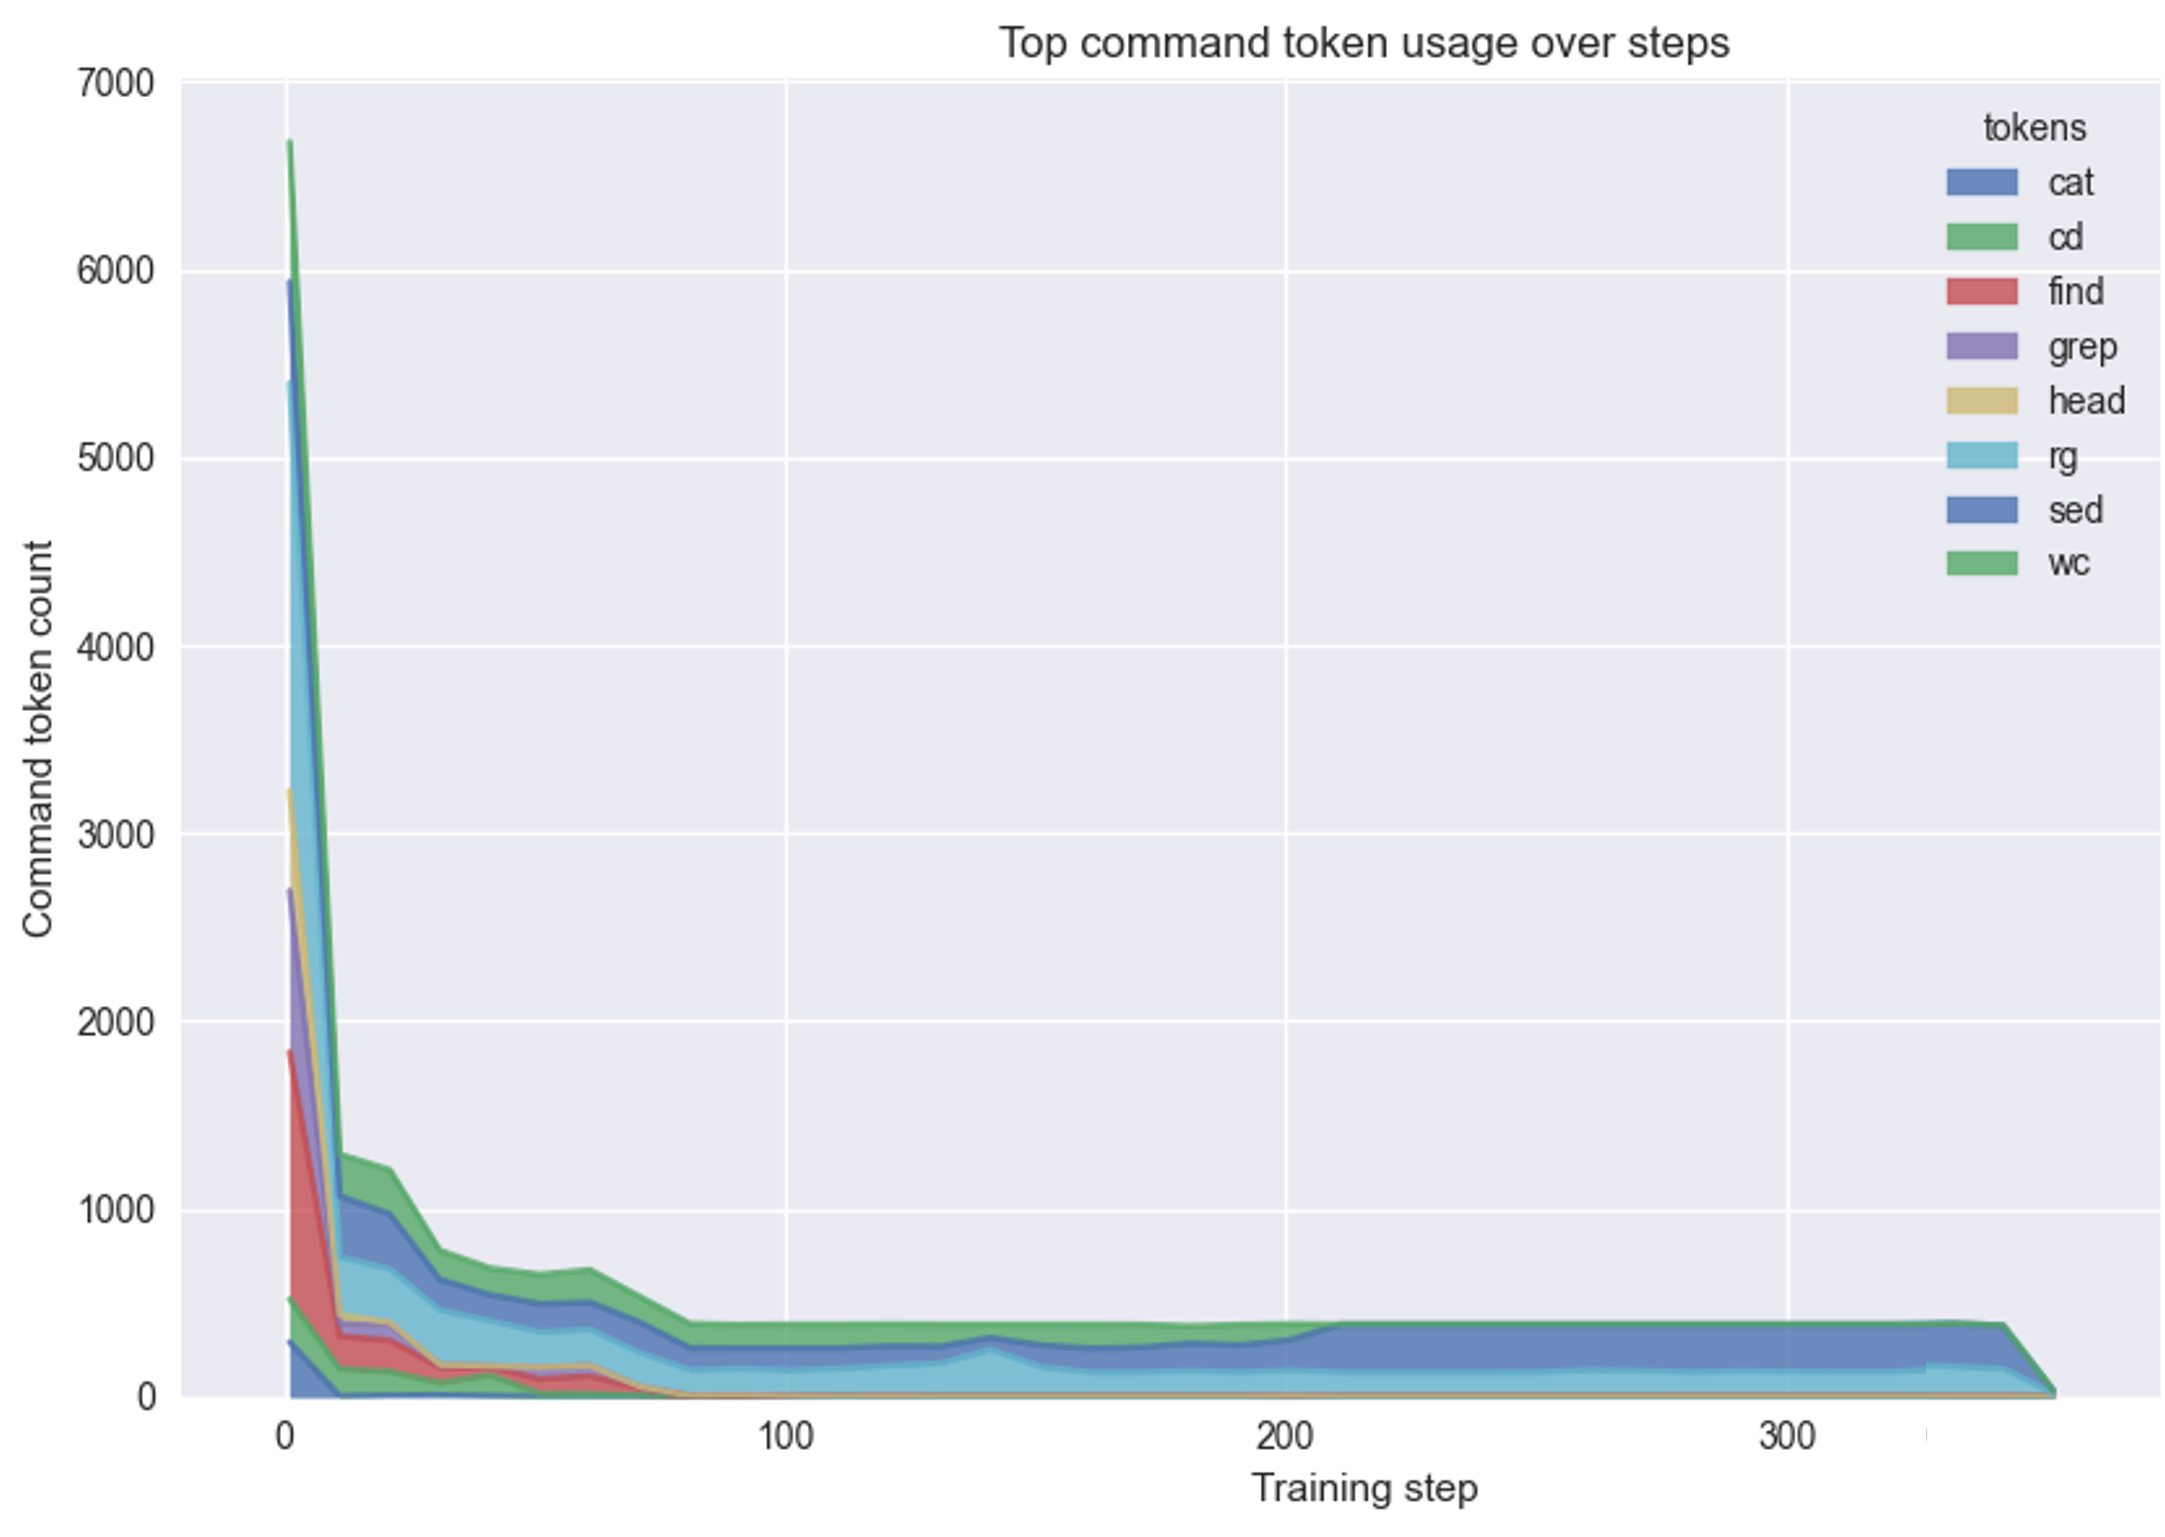
\includegraphics[width=0.6\linewidth]{Figures/change.png}
    \caption{Although it starts with using various commands, as training progresses, \methodname quickly learns to only utilize two particular bash commands; \texttt{rg} and \texttt{sed}. This may due to \texttt{rg} capable enough to functionally replace other commands.}
    \label{fig:tool_use}
\end{figure*}
